\documentclass[preprint]{sig-alternate}

\usepackage{hyperref}
\usepackage{microtype}
\usepackage{color}
\usepackage{epsfig}
\usepackage{pslatex}
\usepackage{xspace}

%% reference shortcuts
\newcommand{\figref}[1]{Figure~\ref{#1}}
\newcommand{\secref}[1]{Section~\ref{#1}}

% \|name| or \mathid{name} denotes identifiers and slots in formulas
\def\|#1|{\mathid{#1}}
\newcommand{\mathid}[1]{\ensuremath{\mathit{#1}}}
% \<name> or \codeid{name} denotes computer code identifiers
\def\<#1>{\codeid{#1}}
\newcommand{\codeid}[1]{\ifmmode{\mbox{\ttfamily{#1}}}\else{\ttfamily #1}\fi}


%% Comment out one of these two definitions.
\newcommand{\todo}[1]{\relax}
% \newcommand{\todo}[1]{{\color{red}\bfseries [[#1]]}}

\newcommand{\Popovic}{Popovi\'c\xspace}

\def\floatpagefraction{.9}
\def\dblfloatpagefraction{.9}

%% Bring items closer together in list environments
%% This doesn't work with an optional argument to the list environment.
% Prevent infinite loops
\let\Itemize =\itemize    
\let\Enumerate =\enumerate
\let\Description =\description
% Zero the vertical spacing parameters
\def\Nospacing{\itemsep=0pt\topsep=0pt\partopsep=0pt\parskip=0pt\parsep=0pt}
% Redefine the environments in terms of the original values
\renewenvironment{itemize}{\Itemize\Nospacing}{\endlist}
\renewenvironment{enumerate}{\Enumerate\Nospacing}{\endlist}
\renewenvironment{description}{\Description\Nospacing}{\endlist}

% Reduce indentation in lists.
\setlength{\leftmargini}{.75\leftmargini}


\begin{document}

\title{Verification Games: Making Verification Fun}

% \subtitle{[Project Abstract]}

% \titlenote{A full version of...}}

\author{
Werner Dietl
\qquad
Stephanie Dietzel
\qquad
Michael D. Ernst
\qquad
Nathaniel Mote
\qquad
Brian Walker\\
%
{\normalsize
Programming Languages \& Software Engineering Group,
University of Washington}\\
\url{{wmdietl,mernst,nmote,bdwalker}@cs.washington.edu}
%
\and
%
Seth Cooper
\qquad
Timothy Pavlik
\qquad
Zoran Popovi\'c\\
%
{\normalsize
Center for Game Science, University of Washington}\\
\url{{scooper,zoran}@cs.washington.edu},
\url{timothy.pavlik@gmail.com}
}

\date{}

\maketitle

\begin{abstract}
Program verification is the only way to be certain that a given
piece of software is free of (certain types of) errors --- errors that
could otherwise disrupt operations in the field.  To date, formal
verification has been done manually, by specially-trained engineers.  Labor
costs have heretofore made formal verification too costly to apply beyond
small, critical software components.

Our goal is to make verification more cost-effective by reducing the skill
set required for program verification and increasing the pool of people
capable of performing program verification.  Our approach is to transform
the verification task (a program and a goal property)
into a visual puzzle task --- a game --- that
gets solved by people. The solution of the puzzle is then translated
back into a proof of correctness.
The puzzle is engaging and intuitive enough that ordinary people can through
game-play become experts.

This paper presents a 
% preliminary
status report on the Verification Games
project and our Pipe Jam prototype game.



\end{abstract}

% A category with the (minimum) three required fields
% \category{H.4}{Information Systems Applications}{Miscellaneous}
%A category including the fourth, optional field follows...
% \category{D.2.8}{Software Engineering}{Metrics}[complexity measures, performance measures]

% \terms{Theory}

% \keywords{ACM proceedings, \LaTeX, text tagging}

\iffalse

\section{FTfJP 2012 Call for Papers}

From \url{http://www.comp.nus.edu.sg/~ftfjp/}:

\begin{quote}
Contributions (of up to 6 pages in the ACM 2-column style) are sought
on open questions, new developments, or interesting new applications
of formal techniques in the context of Java or similar
languages. Contributions should not merely present completely finished
work, but also raise challenging open problems or propose speculative
new approaches. We particularly welcome contributions that simply
suggest good topics for discussion at the workshop, or raise issues
that you feel deserve the attention of the research community.
\end{quote}

Dates:

abstract submission: 16 March 2012 (anywhere on Earth)\\
full paper submission: 25 March 2012 (anywhere on Earth)\\
notification: 29 April 2012\\
camera-ready paper: TBD\\
conference date: 12 June 2012\\

\fi


\section{Introduction}

Our aim is to change the way that software is verified, to enable
inexpensive formal verification.  Current approaches that rely on
testing are incomplete.  Current approaches that rely on manual
verification by skilled users are extremely expensive.  
Current approaches are not capable of keeping up with the
current and future rate of software production.

Our approach is to remap the problem into a more accessible
form, and use an engaging game to develop a significantly larger
number of experts capable of solving verification problems in a
remapped domain.  Instead of relying on software engineers, we will
develop a new skilled verification workforce, and use crowd-sourcing
on a much more general audience of people who enjoy the challenge of
playing a game.

The availability of inexpensive formal verification could change the
economics of software verification and validation, making
formally-correct software more cost-effective and thus more
widespread, and  leading to systems that are more reliable and
robust.  
These benefits would extend throughout the software
development lifecycle, because formal specifications make code
maintenance easier and cheaper.


We have built a prototype end-to-end system that takes as input

\begin{itemize}
\item
 an arbitrary Java program and
\item
 a security (or other) property, expressed as a type system
\end{itemize}

\noindent
and produces as output

\begin{itemize}
\item
 a proof of correctness that the program satisfies the security property,
 or
\item
 a specific source location where the program violates the property
 --- that is, where the program may be insecure.
\end{itemize}

This system automatically converts the program and
property into a game that can be played by people with no knowledge of
or training in computing.  When the player finishes a game challenge,
the final configuration of board elements can be translated into a
proof of correctness for the original program.  More precisely, the
board configuration corresponds to a set of type annotations that can
be checked by a type-checker.  The human player can be viewed as doing
type inference.

Because the game is designed to encode the same constraint system as
the type system, if the player solves a level of the game, then the
corresponding annotated program will type-check.  The type-checker
gives a sound guarantee that the type annotations are correct and the
program is secure with respect to the specific security property.

In many cases, the program will \emph{not} type-check ---
equivalently, the game cannot be solved.  There are two main reasons
for this.

\begin{enumerate}
\item
  The program is not secure --- it contains a vulnerability.
\item
  The program is secure, but the reason that it is secure is beyond
  the reasoning abilities of the underlying verification technology.
  Every verification system --- type checking, theorem proving, model
  checking, abstract interpretation, etc.\ --- issues warnings about
  some secure programs.
\end{enumerate}

\noindent
There is no \emph{a priori} way to know which of the two reasons lies
behind a verification failure --- equivalently, an un-solvable game
level.  A fielded version of our system would present each verification failure to a human
verification expert.  The human examines the source code and
determines which of two fixes to apply: change the code to correct the
bug, or add an assertion/assumption indicating that the verification
system should not issue a warning at this particular location.


Even when game-developed experts cannot fully verify
a program, the impact of this paradigm can be significant.  Even
partial verification has great value: it permits the valuable time of
highly-skilled engineers to be focused on the most important parts of
the program.

\subsection{Types for program verification}

\todo{How much motivation should we keep for FTfJP?}

We use pluggable type-checking as the underlying verification
technology.  Type systems are the shining success of program
verification.  Types are used on a regular basis by ordinary
programmers who use them to verify the absence of certain types of
errors.  Programmers write a partial specification in the form of type
annotations, then a type-checker detects potential errors.  No other
formal verification approach has seen such widespread adoption.

Pluggable type-checking provides an excellent foundation from which to
improve upon the limitations of current verification
approaches. Type-checking is \emph{sound}, so it offers a guarantee.
Type-checking is \emph{expressive}: it is formally equivalent
\cite{CurryHoward2006,MartinLoef1984,CoquandHuet1988,Cousot1997,CousotCousot2000,NaikPalsberg2005}
to any other verification technology, including model-checking and
theorem-proving.  Type-checking is already \emph{familiar} to every
developer, and it fits well into the development process.
Type-checking is \emph{modular}: it can be done on each component of a
system individually, making it much more scalable.  Related to the
previous two points, type-checking is \emph{transparent}, which makes
it easy to use: its error messages tend to be clear, and a small
change to the application does not make a large, non-local change to
the type-checking results.  This is relevant both to game players who
will see the error messages in a different guise, and to verification
experts who will take over when the game players get stuck.
Type-checking is \emph{extensible}: even a non-expert can create a
new, custom type-checker that verifies a domain-specific property of
interest; a type system that is extensible in this way is called
``pluggable''~\cite{Bracha2004}.

The downside of type systems is that they tend to be less expressive than
certain other verification techniques.
A type system offers partial verification --- it is designed to detect
a certain class of errors, and the program may still be subject to
other errors.  This is the right way to start, because full formal
verification remains impractical for realistic software.  Furthermore,
type-checkers are powerful and can check a wide range of important
properties.  Our system is built upon the Checker
Framework~\cite{checker-framework-website-20100203},
which has found hundreds of errors in millions of lines of
code~\cite{PapiACPE2008,DietlDEMS2011}.  It can be easily adapted to new
verification problems and comes
with type-checkers that prevent errors due to null pointers;
initialization; map keys; equality tests and interning; incorrect
mutation (side effects); concurrency and locking; fake enumerations;
information flow (trust and security); aliasing; regular expression
syntax; property files; internationalization; the string
representation of data; and many more.  We have mapped the CWE/SANS Top 25
Most Dangerous Software Errors (\url{http://cwe.mitre.org/top25/?2011})
to type systems.

Our system maps source code's typeflow properties
into a network of pipes.
Pipe widths, which are controlled by the player, directly map to type
annotations in programs that can be mechanically checked and provide a
proof of partial correctness.
The constraints and relationships among
game elements are representations of the constraints on program types and
the relationships among program variables.
By playing the game, the programmer is effectively choosing types for
every variable in the program.
This is valuable because general type inference with precise error messages
remains an unsolved problem that can benefit from crowdsourcing.

We believe that humans may have an edge over automated systems in
certain situations, notably when the program is not verifiable.  A
program is unverifiable when it has a bug, or when it is correct for
reasons that are beyond the power of the verification system.  In
either case, the failure is communicated back to an expert, who only
considers cases that the crowd of players cannot resolve.



\todo{
\medskip

The remainder of this paper is structured as follows.
\todo{Write.}}




\section{The Pipe Jam game}
\label{sec:pipejam}


\begin{figure*}
\begin{center}
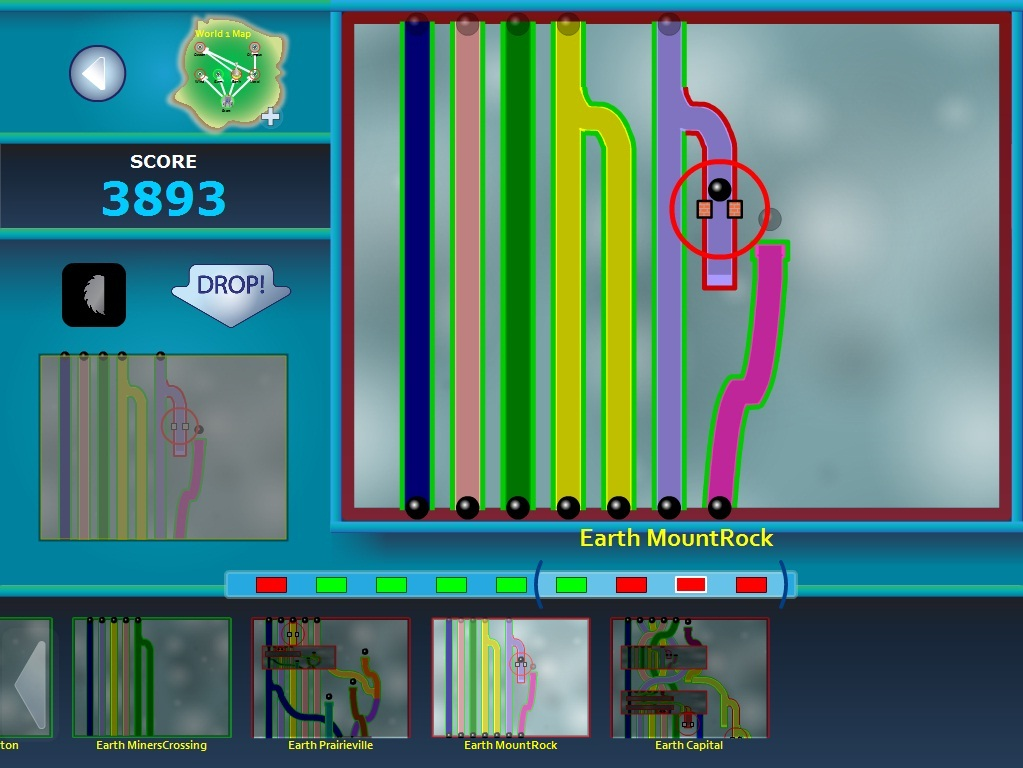
\includegraphics[width=.49\textwidth]{images/allUI-world1}%
\hfill%
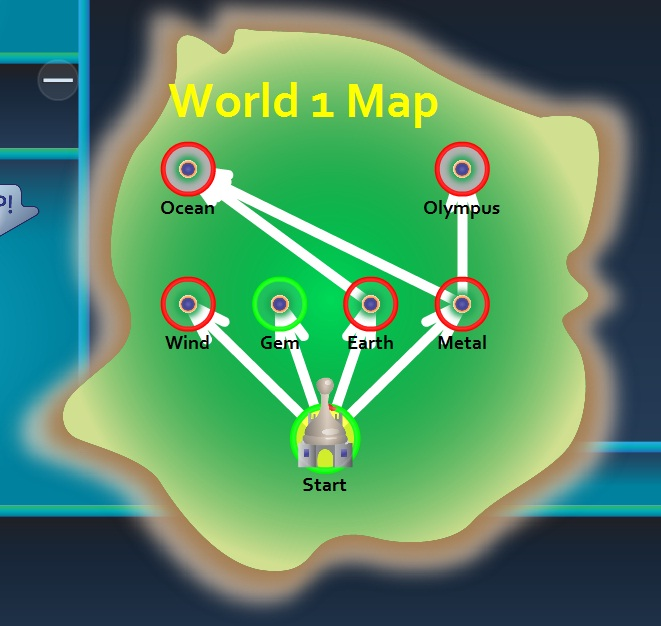
\includegraphics[width=.35\textwidth]{images/world-map}
\end{center}

\caption{
  A view of the Pipe Jam verification game being played.  The underlying
  verification problem is to prove that a part of our system itself is free of
  null pointer errors.
  \newline
  The left screenshot shows the player's view of the game.  In the
  upper right is the board that the player is currently working on
  (named ``Earth MountRock'').  The bottom portion of the screen shows
  thumbnails of all the other boards in the current level, together
  with a concise summary of which boards are solved and which are
  unsolved (the row of red and green rectangles).  The thumbnail at
  center left is for panning, which is not needed in this example.
  Above it are controls for adding a buzzsaw and for viewing an
  animation; the current score; and a back button and the collapsed
  world map.
  \newline
  The right screenshot shows the world map in its expanded state.  The
  world map shows named levels and the dependencies between them, and 
  permits the player to navigate to a new level.
}
\label{fig:game-overview}
\end{figure*}


Figures~\ref{fig:game-overview}, \ref{fig:game-detail},
and~\ref{fig:game-buzzsaw} show screenshots of the Pipe Jam game.  The
screenshots show Pipe Jam being used to verify that a part of our system
itself is free of null pointer errors.  We now explain the figures.

Pipe Jam presents the game player a set of related ball-and-pipe
puzzles.  Each pipe is either narrow or wide, and the player is
allowed to control the width of some pipes.  Each ball is either small
or large.  A small ball can roll down any pipe without obstruction.  A
large ball can roll down a wide pipe, but gets stuck if it ever tries
to roll down a narrow pipe.  The player's goal is to ensure that the
balls never get stuck.

A player might try to make all pipes wide, but this does not work
because some pipes are narrow and cannot be adjusted.  (This is
sometimes represented as an obstruction, or pinch point, that only
permits a small ball; see Figures~\ref{fig:game-overview},
\ref{fig:game-detail}, and~\ref{fig:game-buzzsaw} for examples of
pinch points.)  Likewise, some balls are large and cannot be adjusted;
see Figures \ref{fig:game-detail} and~\ref{fig:game-buzzsaw} for
examples of balls (atop gray pipes) that are fixed to be large.  The
puzzle is solved when the player has chosen widths that are consistent
with all the constraints, including both fixed sizes and which pipes
flow into one another.

The basic idea behind Pipe Jam is simple and lends itself to quick
learning and enjoyable play.  We now explain some additional game
mechanics that add interest and challenge.  (These game mechanics are
much easier experienced than textually described.)

\begin{description}

\item[Boards and levels]
  A Pipe Jam game is divided into boards, levels, and worlds.  A board is a
  single network of pipes.  A level consists of a set of boards.  The level
  is solved when all of the boards in it have been solved.  As explained
  below (``linked pipes''), actions on one board can affect another board:
  the player must solve all of them simultaneously, not one after the other
  independently.

\item[Levels and worlds]
  A world consists of multiple levels.  A player proceeds through the
  world, ``conquering'' each level one by one.  As shown in the world map
  of \figref{fig:game-overview}, the levels depend on one another,
  which constrains the order in which the player may solve them.  It may
  sometimes be necessary for a player to backtrack to a previous level to
  find a better solution for it, in order to solve a subsequent level.
  ``Embedded networks'' below explains how boards and levels depend on one
  another.

\begin{figure*}
\begin{center}
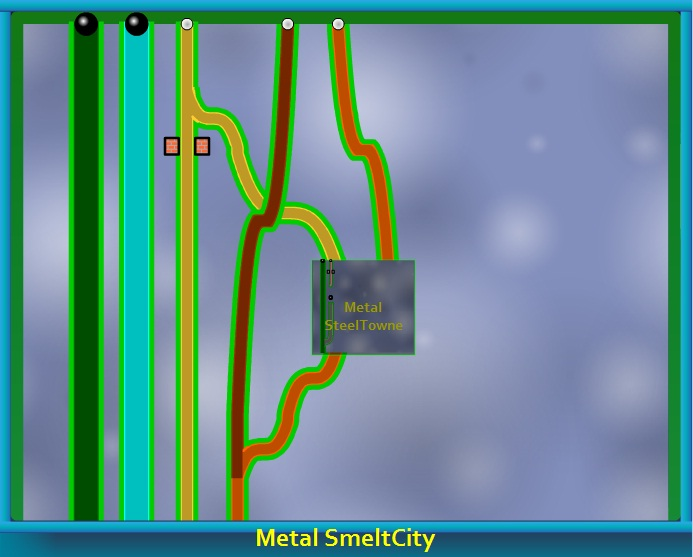
\includegraphics[width=.49\textwidth]{images/world1-subnetwork}%
\hfill%
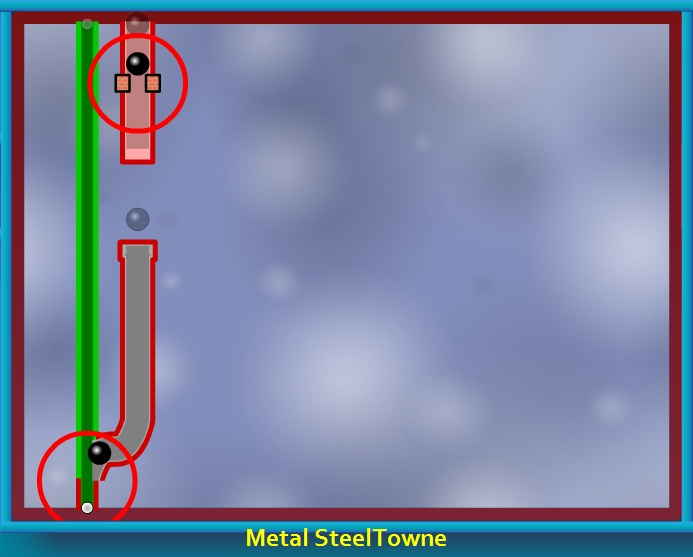
\includegraphics[width=.49\textwidth]{images/world1-merge-and-pinch}
\end{center}

\caption{
  Detail of two boards from the Pipe Jam game shown in
  \figref{fig:game-overview}.  The left board demonstrates wide and
  narrow pipes, pinch points, a merge (near the bottom center), and a
  subnetwork.  The right board demonstrates two collisions, each of which
  prevents the game from being solved.  At the top, a large ball
  collides with a pinch point.  At the bottom, a wide ball gets stuck
  trying to merge into a narrow pipe.  The collisions are highlighted by
  red circles.  A pipe segment is outlined in green if it contains  no
  collision, and in red if it contains a collision.
  The gray pipe on the right board cannot be adjusted in width.
}
\label{fig:game-detail}
\end{figure*}


\item[Linked pipes]
  All the pipes of a given color (in a board or an entire level) have the
  same width.
  (An example is the two orange pipes in \figref{fig:game-detail}.)
  When the player changes the width of one of these pipes,
  then it also changes the width of all the other pipes of that color.
  When the player changes the width of a give pipe, that change may solve
  one board on a level but unsolve a different, previously-solved board on
  the same level.  The player's challenge is to find a set of pipe widths
  that simultaneously solve the entire level.

\item[Embedded networks]
  One network can contain another network as a subcomponent.  For example,
  in \figref{fig:game-detail}, the left board ``Metal SmeltCity''
  contains another board ``Metal SteelTowne'' as a subcomponent.  When
  balls roll through SmeltCity to the subcomponent, they next traverse the
  subcomponent to its end before returning to SmeltCity.  Changes to the
  width of the input or output pipes of the subcomponent, Metal SteelTowne,
  can cause collisions in SmeltCity.  This is another example of
  relationships among boards that the player must satisfy.
  The embedded network may come from the same level, or any level that
  does not follow the current one on the world map.  Mutually dependent
  classes can be processed in either order.  In the worst case, a player
  may need to visit each one multiple times.

\item[Buzzsaws:  Exceptions to the laws of physics]
  Not every Pipe Jam game is solvable.  It is possible that every
  combination of pipe widths yields at least one collision.  To let players
  proceed in this case, Pipe Jam contains a ``cheat'' --- the buzzsaw ---
  that any player is allowed to use at any time.  A buzzsaw converts any
  ball that passes by it to a small ball, which can then fit through any
  pipe.  See \figref{fig:game-buzzsaw} for an example.
  It would be possible to solve any level using sufficiently many buzzsaws,
  without changing the sizes of any pipes.  However, placing a buzzsaw
  costs a large number of points, so players desire to use as few buzzsaws
  as possible.
  \todo{I think this last sentence is the first mention of
    points. Maybe this should be introduced earlier?}

\end{description}



\begin{figure*}
\begin{center}
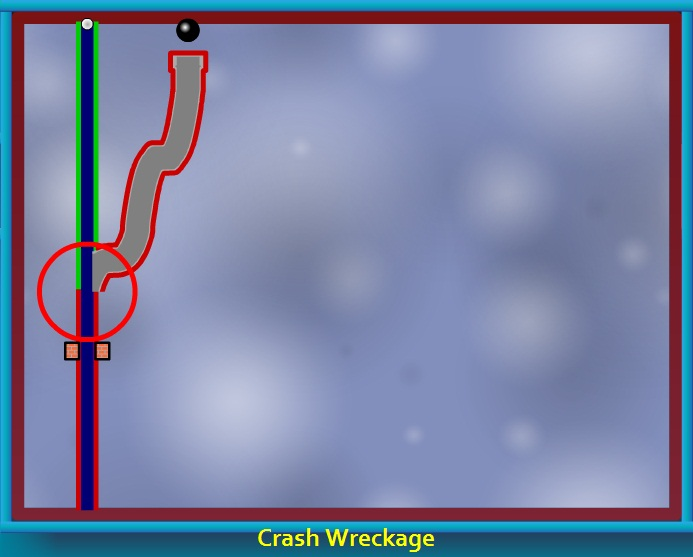
\includegraphics[width=.49\textwidth]{images/unsolvable-pre-buzzsaw}%
\hfill%
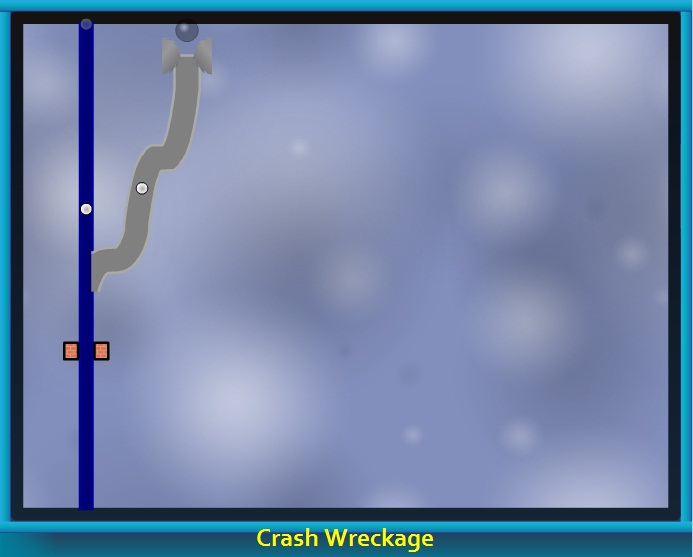
\includegraphics[width=.49\textwidth]{images/unsolvable-post-buzzsaw}
\end{center}

\caption{
  The left board is unsolvable.  The gray pipe cannot be adjusted in width,
  and the black ball will get stuck trying to merge into the narrow blue
  pipe.  Even if the blue pipe were made wide, the black ball would still
  get stuck at the pinch point.
  \newline
  The right screenshot shows how to solve the board by placing a buzzsaw.
  A buzzsaw cuts any ball that passes through it.  The animation captured
  in the right screenshot shows that the large ball has been transformed
  into a small one after passing through the buzzsaw, and the level is
  solved.  Placing a buzzsaw reduces the player's score, so players will
  try to solve their puzzles with the minimal number of buzzsaws.
}
\label{fig:game-buzzsaw}
\end{figure*}


The natural modularity of object-oriented programs, which are composed
of classes that are composed of methods, makes our game attractive to
casual gamers who can do a little bit of work and then later come back
to the game.  However, it is possible for interrelations to cross
levels --- because of global variables that are used in multiple
classes, or because of calls from one class to another.


In \figref{fig:game-overview}, the player has not yet solved the
game.  The outline color of each board and thumbnail (green or red)
indicates whether it is solved.  At any time, the player can animate
the networks, making balls flow along them and seeing the result, but
the colored borders give immediate visual feedback.  We plan to
support two different types of animations: a type-theoretic one that
reflects what the underlying program verification tool can establish (this
is already implemented),
and an execution-based one that illustrates what the program actually
does on some set of real executions.  The latter is more precise but
incomplete~\cite{Ernst2003:WODA}, so the two approaches are
complementary.


\section{Mapping a program and a property into the Pipe Jam game}

We now explain, at a high level, our algorithm for translating a
verification problem --- that is, a program and a property that may be
true of the program --- into an instance of the Pipe Jam game.

A Pipe Jam game is analogous to a dataflow network for a program.
In this analogy, each ball represents a value, each pipe 
represents a variable, and assignment between variables is represented
as one pipe flowing into another.  In actuality, a Pipe Jam game represents
a relation we call ``type flow''.  For example, a parameterized type
\codeid{Map<String, Integer>} would be represented by three pipes, one (or
more) each for the type qualifiers on \<Map>, \<String>, and \<Integer>.
The three pipes need not always flow in parallel, depending on how the code
uses values of the given type.

The width of a pipe stands for the type of the variable that the pipe
represents.  These are not the underlying Java types, but the security
properties that are represented in the pluggable type system.
For
concreteness consider a nullness type system: a wide pipe represents a
variable that is permitted to contain the value \<null>, and a narrow
pipe represents a variable that is guaranteed to be non-null.  More
generally, for a two-element type system, the wide pipe represents the
supertype and the narrow pipe the subtype.

Unmodifiable pipes stand for constraints arising from the source code.
For example, a field dereference such as \<x.f> requires that the
reference \<x> be non-null (narrow).  The literal \<null> yields a
large ball, and a \<new> expression yields a small ball.  Similar
constraints arise from secure sources and untrusted sinks in a
security type system.

Each board represents a single procedure or method.  Each level
represents a class.  An embedded board represents a procedure call.
When there is a procedure call to a pre-annotated library routine,
then its constraints are integrated directly into the network, to
avoid a proliferation of subcomponents in the network.

The world map is a dependence graph among classes or, equivalently, a
call graph.  It ensures that callees are annotated before callers,
though it accommodates mutual dependences.

Linked pipes that are of the same color represent different
occurrences of the same variable or of two variables whose types must
be identical.  For example, a global variable or a class's fields flow
to every method and thus appear on every board, but each global
variable or field has only a single type that must be consistent
across all methods in the program.

A buzzsaw represents an assumption/assertion about a given value --- for
example, a loophole, suppressed warning, or trusted cast in the type
system.  A programmer writes these to indicate externally-verified
properties.  Human insight is likely to be
more effective than any inference tool, as evidenced by the sorry
state of error messages for type inference systems.  Once our system is
fielded, then whenever many
players, or a known successful player, uses a buzzsaw, a trained
programmer can examine the code to understand the code at that
location property.  The programmer determines whether the code is
correct and needs a trusted assumption, or the code has a bug and
should be fixed.  The game players have focused the scarce, expensive
resource (expert programmer time) exactly where it is most
needed.\footnote{One can imagine other game mechanics for expert
  players, such as the ability to rewire the network.  This
  corresponds to changing the logic of the program or rearranging
  assignments.  It must be done in a way that respects the underlying
  Java types.  Like the buzzsaw, this mechanism would reduce the
  player's score (though in most cases the final score would be more
  than for a complete failure to solve the level), and would be
  verified by a programmer.}


\paragraph{Distinction from dataflow}
The Pipe Jam game does not actually represent dataflow, but a
different concept that we call type flow.  The notion of type flow and our
representation of it are
novel, to the best of our knowledge.  A particular variable may be
represented by multiple pipes if it has a compound type.  For
instance, a variable of type \verb|List<String>| would be represented
by two pipes because two type qualifiers are possible, one on \<List>
and one on \<String>.  On the other hand, other variables would not be
represented at all.  For example, in a nullness type system, all
primitive variables could be elided because a variable of primitive
type (e.g., \<int>) can never hold \<null>.


Although programs very frequently contain loops in their dataflow,
cycles in a single board do not occur, because the network is really
about relationships and flows between types and variables, not just
between specific data values.  Put more technically, it encodes the
type constraints that arise when syntax-directed type constraint
generation is performed on the program.  While still complex, these
are much simpler than the original program.


\subsection{Mapping security vulnerabilities to game puzzles}

\todo{I don't want to list all 25 type systems. Some of these
  descriptions need to be adapted more.}

We have set ourselves the initial goal of formally verifying that Java
programs are free of the errors
listed in the CWE/SANS Top 25 Most Dangerous Software Errors
(\url{http://cwe.mitre.org/top25/?2011}).  It is, in its own words,
``a list of the most widespread and critical errors that can lead to
serious vulnerabilities in software.''

We now discuss how our pluggable type-checking approach can be
instantiated for the errors on the list.  Instantiation requires
creating a \emph{type system} that can detect the error or verify its
absence, and a \emph{mapping} from the type system to our Pipe Jam
game.  The mapping into Pipe Jam is generally straightforward.  We
give three rules that handle most the situations.
%
\begin{itemize}
\item
  Many of the type systems have two qualifiers.  The top qualifier can be
  mapped into a wide pipe and large ball, and the bottom qualifier can be
  mapped into a narrow pipe and small ball.
\item
  When the type system consists of three type qualifiers in a chain (that
  is, $A :> B :> C$, where $:>$ is the supertype relation), then three
  sizes of pipes/balls suffice.
\item
  When the type system contains two types that are incomparable, these
  can be thought of as orthogonal properties of an object.  Examples
  from the nullness type system include whether a reference can be
  null; whether the referent is fully-initialized (versus being
  \<this> within a constructor); and whether the referent is a key in
  a given map (this enables precise analysis of \<Map.get()> calls).
  In this case, a different physical representation is required for
  the different properties.

  We represent the primary or most important property as pipe/ball
  size, and the others as different colors or textures that are
  imposed on the pipe or ball.  As a simple example, a value that is
  not necessarily fully initialized gets gray stippling.  A more
  complex example is whether a value is present as a key in a map.
  Suppose there is a map whose pipe is blue.  Then keys (pipes) that are
  guaranteed to be present in that map get a blue stripe.  This shows
  to the user the relationship between different values.
\end{itemize}

In some cases, a particularly sophisticated type system requires
enhancements to the basic game mechanics.  For example, consider the map
key example above, and recall that \<Map.get> returns non-null only if the
key is in the map and all the map values are non-null.  Representing a call
to \<Map.get> requires a new game widget that takes three input pipes and
one output pipe.  The widget has a narrow output pipe if \emph{both} the
pipe representing the key's type has a stripe of the color of the pipe
representing the map's type \emph{and} the pipe representing the value's
type is narrow.  In our experience with over a dozen pluggable
type-checkers, the nullness type system has the most complexities such as
these, because programmers use \<null> to represent many special cases and
because they can check for it at run time.


\subsection{Simplifying the type constraints and the game puzzles}
\label{sec:simplification}

Even a multitude of game players would have trouble verifying a
5-million-line program with respect to 25 distinct type systems.
Therefore, we propose to simplify the problem before presenting it to the
players.  We will do so by pre-determining the types for a subset of
variables in the program.  Then, the players only need to find types for
the remainder of the program.  We will use the best program analysis tools
available, and then the players will take over.

We expect to significantly reduce the size of the games that players must
solve.  One reason is that some properties are not applicable to many parts
of the program.  Nullness properties are not applicable to primitive types,
which can never have the value \<null>.  Untrusted user inputs are strings,
but most variables in a program are of other types.  A second reason is
that many values are restricted to a small part of the program.  In a
correct program, user input strings are validated near where they are read,
or at least do not flow into strings used for other purposes.  A third
reason is that we will use highly-effective analyses that determine an
answer for most of the program.

The game player is accomplishing the task of type inference:  creating an
annotation for each variable declaration in the program, that gives
additional information about that variable's type.  Examples are whether
the variable is permitted to hold the value \<null>, and whether the
variable is permitted to be mutated.

Type inference tools exist that can infer type annotations for unannotated
code.  Whereas type \emph{checking} is largely a solved problem, type
\emph{inference} emphatically is not.

\todo{Move this paragraph somewhere. Maybe related work?}
Even the most precise available inference tools leave much room for
improvement.  For example, the state of the art tool for inferring
nullness properties is the
Julia~\cite{julia-web-interface,Spoto2008,Spoto10:LPAR,Spoto10,SpotoE2011}
tool for Java.  It can prove about 98\% of all dereferences in a
program to be safe --- that is, it proves that no \<null> value ever
flows to those dereferences, so those dereferences cannot result in a
null pointer exception at run time.  However, this leaves 2\% of
dereferences for a programmer to manually check --- some may be
erroneous code that might fail at run time, but most are probably safe
even though Julia is unable to infer such properties.  A humans'
insight and higher powers of reasoning are required.  As another
example, a state-of-the-art tool for inferring mutability (whether
side effects are permitted/performed) is
Javarifier~\cite{Quinonez2008,QuinonezTE2008} for the
Javari~\cite{BirkaE2004,TschantzE2005,Tschantz2006} type system, but
it, too, suffers imprecision due to its conservative analysis.  An
earlier inference system for
Javari~\cite{GreenfieldboyceF2005,GreenfieldboyceF2007} achieved even
worse results, with precision of about 70\% (compared to Julia's 100\%
precision and 98\% recall).


Automated analysis and crowdsourcing are complementary.  In
particular, we can run the best available practical inference tool
before the player starts, and use that as the initial configuration
that the player attempts to improve.  This leverages human intuition
exactly where it is needed.  In particular, every formal analysis has
a limited vocabulary of properties that it can express, which limits
the properties that it can prove.  It is an unavoidable fact, related
to the undecidability of the halting problem, that for every
conservative (sound) program analysis, there are programs that never
go wrong at run time but that the program analysis rejects as
potentially erroneous.  We hope that humans will be able to overcome
these limitations via higher-level reasoning, pattern-matching, and
heuristics to guide themselves through very large search spaces.

% Are there "verification savants" much as there are for protein folding?



% \section{Game mechanics}
% \label{sec:game}
% 
% \todo{Cut this down to for the FTfJP audience?}
% 
% In order to significantly increase the accessibility of this problem
% to a non-expert audience, and consequently enable crowd-sourcing of
% all people, the game needs to draw in players with no knowledge of
% software verification.  More players will allow us to better determine
% what creative modalities best lead to problem solving, and even more
% importantly, increase the network effect of collectively bringing
% together creative minds. In addition, most of our continuous
% refinement design hinges on the fact that people will be playing the
% game and help us refine the modalities for training creativity.
% Without a large base of game players this design strategy will likely
% not be effective.
% 
% Simply put, to maximize the game-player population, we need to make
% the game fun. This, of course, is a lot easier said than done. Despite
% a large body of work on the topic of what games are fun to play,
% production of a successful game is much more of an art than science.
% Games with a hard problem solving objective in particular are often
% not highly engaging, and tend to capture only a small niche of
% players.  Our team has extensive experience with design of successful
% games in the past.  The Center for Game Science has led the design of
% four games in last two years that collectively gathered over 2 million
% players worldwide.  This is particularly significant considering that
% three of those four games are serious games with learning or
% scientific discovery as the primary design objectives.  Our
% methodology of game design leverages a number of game design
% principles that focus on the maximal adoption of the game:
% %
% \begin{description}
% \item[Competition.] Dynamically updated rankings are known as a
%   singularly most important game play motivator. In our experience
%   with Foldit, the drive to have the highest score has led some
%   players to play Foldit for 11 hours within a single 24 hour trial!
%   As the number of players reaches tens or hundreds of thousands, the
%   effectiveness of a single scoreboard diminishes. To maximize
%   competitive drive, we will have separate scoreboards for a number of
%   different expertise levels. Players that perform well at their skill
%   level advance to the next skill level.
% 
% \item[Collaboration.] Games with unknown hard goals are more fun to
%   play in teams. Teams also tend to amplify the competition aspect of
%   the game. Team-play will be integral part of our game setup. Teams
%   will form their own task distribution strategies. They will be able
%   to share their solutions and strategies, and recruit good game
%   players into the team.
% 
% \item[Demographic neutrality.] To attract the largest possible pool of
%   game players the game needs to be neutral to any specific
%   demographic. For this reason, we want our game to have features of a
%   number of game genres. We want our game to have a minimal ramp-up
%   curve. It needs to be playable for both long and short amounts of
%   time, and it needs to have rewards over short intervals of
%   game-play. These features common to casual games, enable the game to
%   be played by old and young, men and women across many cultures. The
%   game will be available on all major platforms, and, of course, it
%   will be freely available.
% 
% \item[Game Community.] We intend to build a micro-community around
%   this game, with personalized blogs, multiple modes of interaction
%   between players, forums, educational information about specific
%   problems and how the solutions would help the world.
% 
% \item[Encouragement Awards.] The road to successful solutions is
%   likely very long. To maintain the interest of players, the game will
%   provide a variety of incentives and awards along the way. Reaching a
%   certain score may enable new techniques or tool. Players may earn
%   badges, for providing unique solutions that are very different from
%   any others.
% 
% \item[Focus on the first 30 seconds.] According to industry experts,
%   most games are evaluated in the first 30 seconds of the
%   game. Players either abandon the game during that period, or are
%   likely to play a significantly longer period of time. Thus, we will
%   place emphasis on particular playability and attractiveness of the
%   game from the first screen.
% 
% \item[Minimize startup curve.] We also need to make sure that we
%   minimize the time it takes to understand the game goals and learn
%   how to use the interface. We will experiment with in-game tutorials,
%   that provide suggestions to the users based on the techniques that
%   they have not yet used.  As the game is being loaded we can stream
%   the video describing main concepts of game play. We will also
%   publish the videos on YouTube, in hope that the players know as much
%   as possible about the game prior to actually playing the game.
% 
% \item[Making failing fun.] One of the greatest challenges of any game
%   is to make the process of failing fun enough for players to continue
%   with the game. In the context of our game, this means making the
%   play fun enough so that it maximally offsets the lack of progress.
% 
% \item[Playability.] Playability refers to the pure entertainment value
%   of the game experience independent of the performance. It is
%   considered to be an important factor for player retention. We will
%   use our expertise in computer graphics, animation and dynamics to
%   render the game particularly entertaining, to the point that
%   initially just exploring the options would be captivating enough to
%   retain the interest of the player.
% \end{description}
% 
% 
% \subsection{Game-based expert development}
% \label{sec:expert-development}
% 
% A highly-engaging game is capable of drawing in a number of new
% players.  However, if the process of play does not produce increased
% skills, and improvement (both individual and collective) on ability to
% solve verification puzzles, then even a massive population of active
% players will be useless towards the software verification goal.
% Without significant increase of verification puzzle experts worldwide,
% we will not be able to make a quantum leap in the code quality
% compared to the status quo.  This challenge is common to all games
% that attempt to solve hard problems.  Foldit, a proteomics game,
% effectively created the genre of games that solve hard problems.
% Prior to Foldit, it has not been known whether it is even possible to
% elevate human expertise on a particular domain to the point that it
% can disrupt the current scientific process and produce outcomes that
% present significant scientific advances.  In the past few years, based
% on the success of Foldit, several researchers have developed games
% aimed at solving hard problems in science and engineering.  Still to
% date, Foldit remains the only game with strong indisputable evidence
% of emergent expertise and outcomes that advanced the science
% (discoveries published in three Nature papers published in under 2
% years).
% 
% The only way to accurately assess the emergence of expertise in the
% player population is to measure their performance on hard verification
% puzzles.  Once assessed, the key game design question is how to modify
% the game towards improved performance.  Our team has shown with the
% Foldit game that our approach of iterative game sensitivity analysis
% is capable of finding modifications that significantly improve
% performance over time.
% 
% 
% \subsection{Open Verification Puzzles: Crowdsourcing programs}
% 
% Once we have determined the efficacy of the game towards verifying our
% programs, we will commence the stage of open-software challenges.  At
% that point we will create a game portal where anyone can submit the
% software they would like to be verified.  The submittal process will
% have two very important aspects: (1) software translation will be done
% on the client side, assuring all submitters that their entire code has
% been converted into an uninterpretable representation
% (privacy-preserving), (2) the verification process will be free,
% removing any initiation hesitation.
% 
% Our team will serve as a curator of puzzles, selecting ones that would
% be most informative to the effectiveness of the game, and those that
% would contribute the most towards collective mastery development of
% the players.
% 
% We will also enable third-parties to provide monetized incentives
% towards verifying their own programs creating the market and
% contributing to the incentives of existing game experts.


% \section{Implementation}
% \label{sec:impl}
% 
% \todo{What is a good title for this section? Should it come earlier?}
% 
% \todo{We could give an overview of the constraint generation from
%   \cite{DietlEM2011} and/or describe the workflow on the website?}
% 
% 
% Because we would not have time to create 25 new type inference tools, we
% will instead create a new type inference framework for this project.  It
% will generalize existing specific type inference tools in the same way that
% our Checker Framework tool generalized existing specific type-checking
% tools.  This will make it easy to quickly create a type inference tool that
% corresponds to a given type system.
% 
% We will build upon our experience with the Checker Framework, and also
% upon our other previous work in type inference, which is reviewed
% below.
% 
% Much of the proposed work for the type inference framework mirrors
% that we have done for the Checker Framework, our type checking
% framework: supporting rich type hierarchies and backward
% compatibility; infrastructure that manages generics instead of forcing
% the inference system designer to do so; declarative syntax for
% inference rules including a common syntax with that for type checkers;
% etc.  One that is worth mentioning is implementing multiple individual
% checkers for maximally different type systems before finalizing the
% framework design.  This worked very well while building the Checker
% Framework, which has since evolved nonetheless.  Finalizing the
% framework too early suffers the risk of being over fitted to one
% specific type system or view of type inference.  The remainder of this
% section focuses on issues specific to type inference.
% 
% The type inference framework will share code with the Checker
% Framework.  This reduces effort, increases reliability and
% functionality, and makes the system more familiar to users.  The
% Javarifier design, implementation, and evaluation taught us a lot
% about both the algorithms and how to build a type inference system,
% but we do not expect to reuse any of the Javarifier code --- we will
% start over from scratch to build a greatly improved system.  (The
% Javarifier implementation will be extremely useful for regression
% testing, however.)  The result is that a programmer will be able to
% construct a type inference system as easily as a type checker --- and
% with much the same code.  As with the Checker Framework, a programmer
% will use declarative mechanisms where possible, and will override a
% few methods when the type system was not anticipated by the framework.


\section{Related work}
\label{sec:related-work}

In the following we discuss related work along two axes: type
inference and program verification.

\todo{This section is way too detailed.}


% \subsection{Type inference}
% \label{sec:type-inference-previous}
% 
% \todo{This is a review of our previous work, not general work on type
%   inference. Change title or contents?}
% 
% Our type inference framework will take advantage of insights we have
% gained during several previous projects.
% 
% The most closely related previous experience is building an inference
% tool \cite{DietlEM2011} for an ownership type system
% \cite{DietlPhD09}.  One particular problem with the inference of
% ownership type systems is that multiple valid solutions exist and that
% the programmer needs to be able to express design intent.  Our tool
% generates type constraints by traversing the abstract syntax tree and
% encodes heuristics by giving weights to solutions.  It then encodes
% the constraints as a Max-SAT problem and uses an off-the-shelf solver
% to find a solution with an optimal weighting.  Our inference is a
% tunable, iterative approach, in which the programmer finds the desired
% annotations by tuning the heuristics, adding partial annotations, and
% fixing bugs in the program.
% 
% We will also build on our previous experience with the Javarifier type
% inference algorithm~\cite{Tschantz2006,QuinonezTE2008} for the Javari
% language for reference immutability~\cite{BirkaE2004,TschantzE2005}.
% A Javari type-checker is implemented using Java annotations and the
% Checker Framework~\cite{PapiACPE2008}.  Javarifier is sound (its
% results type-check) and precise (making any more references
% \codeid{@Readonly} causes the program not to type-check).  Javarifier
% handles the full Java language including generics, wildcards, and
% arrays.  It infers a rich, practical type system that includes
% parametric polymorphism over mutability and permits excluding fields
% from an object's abstract state.  Javarifier~\cite{Tschantz2006} is
% orders of magnitude more scalable than other type inference systems
% such as JQual~\cite{GreenfieldboyceF2007}, even though JQual handles
% less of Java and less of Javari.  There are algorithmic reasons for
% this, such as that Javarifier employs context sensitivity exactly
% where the program needs it.  For example, it takes advantage of
% generics that are already in the program (or that are inferred by a
% separate tool~\cite{DonovanKTE2004,KiezunETF2007}), in addition to
% using more general context-sensitivity elsewhere.  There are also
% implementation reasons, such as better abstractions and handling more
% of the Java language.
% 
% The Checker Framework already supports flow-sensitive analysis, which has
% many benefits.
% %
% Flow-sensitivity reduces the programmer annotation burden.  We have shown
% that in many cases flow-sensitivity can be combined with careful choice of
% defaults to achieve the same effect as local type inference, at a fraction
% of the algorithmic cost~\cite{PapiACPE2008}.
% %
% Flow-sensitivity has many other benefits as well.
% %
% Flow-sensitivity can eliminate the need to introduce local variables.
% %
% Flow-sensitivity
% is critical for some type systems, such as one for checking nullness.
% (This is because many methods return null under special circumstances, and
% because null has so many different special meanings in different
% applications.)
% %
% The Checker Framework's flow-sensitivity framework was general enough to
% extend with a few lines of code to create a proof-of-concept typestate
% analysis.
% 
% We have also implemented a combined static and dynamic mutability
% analysis~\cite{ArtziKGE2007}.  Its judicious use of expensive static
% analyses makes it competitive with much more sophisticated
% analyses~\cite{SalcianuR2005} at a fraction of the cost.  The static
% component soundly infers immutability, and the novel dynamic component
% soundly infers mutability.  Overall, the approach combines multiple
% lightweight, scalable analyses in stages, with each stage refining the
% overall result.  The resulting analysis is scalable and combines the
% strengths of its component analyses.
% 
% In previous work, we inferred abstract types~\cite{GuoPME2006} via a
% dynamic unification-based analysis.  This indicates the variables that are
% used together or are used in different ways.  It refines the types that
% a programmer writes in the source code, much as type qualifiers also refine
% the types that a programmer writes in the source code.  We have performed
% preliminary experiments that showed that these partitions of the code are
% usually consistent, and that when they are not consistent they often
% indicate a problem.
% 
% Finally, we have used static syntax-directed type constraint generation for
% refactoring~\cite{DonovanKTE2004,KiezunETF2007}.  The essential insight is
% that the program as written is only one of many possible solutions to the
% type constraints.  This is precisely the case in type inference for a
% pluggable type system as well.  An unannotated program is one solution in
% which no reference is (guaranteed to be) immutable, or non-null, or
% interned.  But other solutions exist in which guarantees can be made.
% These result in a modified program, either by refactoring or by introducing
% type qualifiers.
% 
% 
% \subsection{Program verification}

Currently, there is no rapid, cost-effective approach for establishing that
an application is safe.  Testing and dynamic analysis are pragmatic and
often effective, but they are unsound because tests are never guaranteed
to exercise all program behaviors.
Another common approach is to manually inspect the source code
or machine code, relying primarily on expert human insight augmented by
relatively low-level tools.  This approach is slow, costly, and
error-prone; automation, as we propose, is preferable.  Another possible
approach is formal verification via model-checking, theorem-proving, and
similar technologies.  These approaches are attractive because they have
the ability to produce a proof of correctness that guarantees a particular
property.  However, they are not practical, for several reasons.  They
suffer a high false alarm rate, which is caused by analysis approximations
that are a necessary compromise to make a sound analysis scale.  For
similar reasons, the properties they can prove are relatively weak, and in
practice, loopholes/assumptions are required in strategic places.  Even so, they
require a high skill level --- 6 months of training is considered a lower
bound to use a theorem-prover, and model checkers also have a significant
learning curve.

Space restrictions permit us to mention related work only briefly.

\emph{Automatic verification} is the gold standard.  One good example is
Saturn~\cite{AikenBDDHH2007}, a precise and scalable static analysis
tool that was used to verify cast safety of 6 million LOC from the Linux
kernel.
This is an impressive tool; however, custom analyses are written in a
targeted logical programming language and require deep understanding
of the analyses.
Our approach is more flexible and general, and admits both simpler and more
sophisticated analyses, all written in Java.

\emph{Interactive verification} of software has also seen recent impressive
results.
The formal verification of an L4 operating system
microkernel~\cite{Klein_EHACDEEKNSTW_10}
is a recent breakthrough of manual formal verification.
The 8,700 lines of C code of an L4 microkernel were verified using the
Isabelle/HOL interactive proof assistant~\cite{Isabelle2002}.
The group co-designed the kernel and proof and started from scratch;
they developed a Haskell prototype that was manually translated into a
high-performance C implementation.
The verification effort is huge:  over 22 person-years of effort by
highly-trained researchers.
Another recent example is the manual verification of the Compcert C
compiler~\cite{Leroy2009} using the Coq proof assistant~\cite{Coq2004}.
The compiler is written in 42,000 lines of Coq (note that this is both
the implementation and proof) and took about 3 person-years.
In contrast, by continuing to use Java as underlying development
language and extending the type system with expressive, high-level
types, we hope to allow even average software engineers to verify
their software, with the help of the crowd.

A shining example of \emph{software model checking}
is the SLAM/Static Driver Verifier (SDV)
tool~\cite{BallMMR2001,BallBKL2010,BallLR2011} from Microsoft, which
is used to show the correctness of kernel-mode drivers and is a standard
part of the development process.
The tool is applied to device drivers of between 1K and 30K LOC\@.
This success is due to clever ideas, good engineering, and not least the
choice of a very constrained domain with specific properties to check.  Our
goals are considerably more general.

\newcommand\astree{Astr\'{e}e}

\emph{Abstract interpretation}~\cite{CousotCousot1977,Cousot2007}
serves as a foundation for several verification approaches.
The \astree{} tool is used to show the absence of runtime errors in
safety-critical, embedded control code of up to a million lines of C
code.
\astree{} runs not on
programmer-written source code, but on generated code, which uses a limited
subset of C (\astree{} does not handle expressions with side effects,
dynamic memory allocation, or recursion) and has properties
that make the specific properties that \astree{} checks easy to verify.


% Currently, there is no rapid, cost-effective approach for establishing that
% an application is safe.  Testing and dynamic analysis are pragmatic and
% often effective, but they are unsound because tests are never guaranteed
% to exercise all program behaviors.
% Another common approach is to manually inspect the source code
% or machine code, relying primarily on expert human insight augmented by
% relatively low-level tools.  This approach is slow, costly, and
% error-prone; automation, as we propose, is preferable.  Another possible
% approach is formal verification via model-checking, theorem-proving, and
% similar technologies.  These approaches are attractive because they have
% the ability to produce a proof of correctness that guarantees a particular
% property.  However, they are not practical, for several reasons.  They
% suffer a high false alarm rate, which is caused by analysis approximations
% that are a necessary compromise to make a sound analysis scale.  For
% similar reasons, the properties they can prove are relatively weak, and in
% practice, loopholes/assumptions are required in strategic places.  Even so, they
% require a high skill level --- 6 months of training is considered a lower
% bound to use a theorem-prover, and model checkers also have a significant
% learning curve.
% 
% 
% We now discuss selected previous work in static program analysis.
% 
% 
% 
% Program verification is a grand
% challenge of computer science~\cite{Hoare2003}, requiring a considerable, coordinated
% research effort.
% Tony Hoare initiated the VSTTE (Verified Software: Theories,
% Tools and Experiments) conference series to enhance discussion,
% collaboration, but also competition, between the different research
% approaches.
% %
% After early optimism about the power of static analysis came a phase
% of disillusionment in which research focused on testing instead.
% In recent years a few high-profile static verification successes
% rekindled interest.
% One contributing factor was the increased computational power of
% Boolean Satisfiability (SAT) and Satisfiability Modulo Theories (SMT)
% solvers over the last decade.
% Even though SAT is known to be NP-complete, practical instances can be
% solved efficiently.
% Building on Kautz and Selman's seminal ideas~\cite{KautzS96,KautzSM96}, the
% \todo{PI (Ernst)} was the first to build a system that solves a problem by
% automated translation to SAT~\cite{ernst-ijcai97}.
% 
% 
% \emph{Automatic verification} is the gold standard.  One good example is
% Saturn~\cite{AikenBDDHH2007}, a precise and scalable static analysis
% tool that was used to verify cast safety of 6 million LOC from the Linux
% kernel.
% This is an impressive tool; however, custom analyses are written in a
% targeted logical programming language and require deep understanding
% of the analyses.
% Our approach is more flexible and general, and admits both simpler and more
% sophisticated analyses, all written in Java.
% %
% The recent Verified Software Competition \cite{KlebanovEA11} contains
% pointers to several current program verification approaches and
% compares their strengths and weaknesses.
% ESC/Java \cite{Detlefs-etal98,FlanaganLLNSS02,CokK2004} is a well-known
% (unsound) extended static checking system for Java that uses an automated
% theorem prover, Simplify~\cite{Nelson80,DetlefsNS2003}, under the hood.
% There are also considerable contributions from Microsoft Research, for
% example the Spec\# \cite{BarnettEA10,LeinoMueller09a} language,
% the Boogie intermediate verification language~\cite{Boogie}, and the
% Z3 theorem prover~\cite{Z3}.
% In many of these automatic verification tools, instead of working on a
% proof in a separate tool, additional annotations have to be added to
% the source code until the automatic prover can successfully proof all
% properties.
% In our approach, simple type annotations, supported by type inference,
% will make verification simpler for developers.
% A theorem prover can be more powerful than type-checking, so we will
% augment the latter with additional analyses.
% 
% 
% \emph{Interactive verification} of software has also seen recent impressive
% results.
% The formal verification of an L4 operating system
% microkernel~\cite{Klein_EHACDEEKNSTW_10}
% is a recent breakthrough of manual formal verification.
% The 8,700 lines of C code of an L4 microkernel were verified using the
% Isabelle/HOL interactive proof assistant~\cite{Isabelle2002}.
% The group co-designed the kernel and proof and started from scratch;
% they developed a Haskell prototype that was manually translated into a
% high-performance C implementation.
% The verification effort is huge:
% overall 200,000 lines of Isabelle script needed to be written;
% approximately 2.5 person years were spent on the specification and
% implementations of the Haskell and C version; and
% 20 person years were spent on proofs, of which 11 person years were
% L4-specific, and the remaining 9 person years for the development of the
% verification framework and proof strategies. 
% The high level of necessary qualification of the involved team can
% also not be ignored.
% Another recent example is the manual verification of the Compcert C
% compiler~\cite{Leroy2009} using the Coq proof assistant~\cite{Coq2004}.
% The compiler is written in 42,000 lines of Coq (note that this is both
% the implementation and proof) and took about 3 person-years.
% In contrast, by continuing to use Java as underlying development
% language and extending the type system with expressive, high-level
% types, we hope to allow even average software engineers to verify
% their software.
% 
% 
% The shining example of \emph{software model checking}
% is the SLAM/Static Driver Verifier (SDV)
% tool~\cite{BallMMR2001,BallBKL2010,BallLR2011} from Microsoft, which
% is used to show the correctness of kernel-mode drivers and is a standard
% part of the development process.
% The tool is applied to device drivers of between 1K and 30K LOC\@.
% This success is due to clever ideas, good engineering, and not least the
% choice of a very constrained domain with specific properties to check.  Our
% goals are considerably more general.
% % \todo{How big is a typical Android app? I didn't find what the largest
% % programs are they could handle. In the ten-year paper they say the
% % total LOC of all drivers is 450,000, but also that each driver is
% % executed with each rule separately. So the biggest they can handle
% % seems to be closer to 30,000.}
% 
% \newcommand\astree{Astr\'{e}e}
% 
% \emph{Abstract interpretation}~\cite{CousotCousot1977,Cousot2007}
% serves as a foundation for several verification approaches.
% The \astree{} tool is used to show the absence of runtime errors in
% safety-critical, embedded control code of up to a million lines of C
% code.
% \astree{} runs not on
% programmer-written source code, but on generated code, which uses a limited
% subset of C (\astree{} does not handle expressions with side effects,
% dynamic memory allocation, or recursion) and has properties
% that make the specific properties that \astree{} checks easy to verify.
% 
% 
% Several theoretical results put the different approaches to formal
% verification in relation, for example
% types and abstract interpretation
% \cite{Cousot1997},
% model checking and abstract interpretation
% \cite{CousotCousot2000},
% and type systems and model checking
% \cite{NaikPalsberg2005}.
% 
% 
% % Any static analysis of Java programs is complicated by
% % reflection, a dynamic call invocation facility that supports program
% % introspection. Prior work by Livshits et al.~\cite{livshitsreflection}
% % seeks to extend static analysis; adding dynamic checks can further
% % help to ensure safety by validating assumptions.
% 
% 
% Our work uses the Checker Framework for creating custom type systems in
% Java.  Several similar frameworks exist, such as
% Polyglot~\cite{NystromCM2003},
% JavaCOP~\cite{MarkstrumMEMAN2010,AndreaeNMM2006},
% JQual~\cite{GreenfieldboyceF2007}, and
% JastAdd~\cite{EkmanH2007:JastAdd}.
% The latter two do inference as well as checking.
% Limitations of the other frameworks have prevented them from being used to
% build expressive, correct, scalable type-checkers, as the Checker Framework has.
% For a comparison of the frameworks, see~\cite{PapiACPE2008}.
% 
% CQual \cite{FosterFFA99,foster:pldi02}
% is a type qualifier framework for C.
% It provides qualifier polymorphism and inference.
% The framework supports subtyping between the qualifiers and
% well-formedness constraints for types, both specified declaratively
% using a configuration file. Adding imperative type checks is not
% possible without modifying the framework itself.
% The framework has been used --- by its authors --- for const, locking, and
% user/ker\-nel\discretionary{-}{}{}level bug detection.
% CQual can be considered an early success story for using pluggable
% type systems to show correctness properties.
% However, by providing simple extensibility for the verification
% engineer, we hope to make our tool more widely applicable.



% \section{Conclusions}
% 
% 
% \section{Acknowledgments}
% 
% Mention funding?


\enlargethispage{10pt}

\bibliographystyle{abbrv}
\bibliography{2012-pipejam,bibstring-abbrev,ernst,invariants,other,types,pag,sideeff,refs}


\balancecolumns


\end{document}


%%% Local Variables: 
%%% mode: latex
%%% mode: auto-fill
%%% mode: flyspell on
%%% End:
